\documentclass[12pt]{article}

% Package imports
\usepackage[a4paper, margin=1in]{geometry} % Set page size and margins
\usepackage{amsmath, amssymb} % For mathematical symbols and equations
\usepackage{graphicx} % For including graphics
\usepackage{caption} % For customizing captions
\usepackage{cite} % For proper citations
\usepackage{hyperref} % For hyperlinks
\usepackage{float} % For positioning figures
\usepackage{setspace} % For line spacing
\usepackage{datetime}
\usepackage{calc}

% Title and author
\title{WanderLust: A Comprehensive Report}
\author{Eazdan Mostafa Rafin \\Roll: 2003055 \\ Department of Computer Science and Engineering, RUET \\ 2003055@student.ruet.ac.bd}
% \date{January 07, 2025}

\begin{document}

% Title Page
\maketitle

% Keywords
% \textbf{Keywords:} WanderLust, booking platform, travelers, property owners, technology stack

% Sections
\section{Introduction}
WanderLust is a modern, user-centric booking platform that connects tourists and property owners. It is designed to meet a variety of demands and provides customers with a seamless experience when searching for accommodations ranging from fancy hotels to comfortable apartments. WanderLust offers a variety of options to meet your needs, whether you're looking for a relaxing vacation, a business trip, or a one-of-a-kind travel experience.
The portal allows hosts to easily list their properties, whether they run a huge, prestigious hotel or a tiny flat that they want to rent out temporarily. Travelers, on the other hand, benefit from an easy-to-use interface that allows them to search by location, read thorough descriptions, and book with a few clicks.
WanderLust is designed to make vacation planning easier, more accessible, and customized. It seeks to establish a community-driven environment in which property owners and guests collaborate to produce unique and memorable experiences. WanderLust prioritizes convenience, inclusiveness, and variety to guarantee that everyone, from budget travelers to luxury seekers, may discover their ideal stay.


\section{Goals and Objectives}
\begin{itemize}
    \item Simplify the booking experience for travelers.
    \item Hosts can list their properties on the platform.
    \item Hosts can include both large, luxurious hotels as well as apartment owners looking to rent out their space temporarily.
    \item The platform is designed to be easy and accessible for both travelers and hosts.
\end{itemize}

\section{Target Audience}
WanderLust's target audience comprises travelers looking for a variety of housing options as well as hosts willing to sell and monetise their homes, which range from individual flats to luxury hotels.


\section{Key Features}
\subsection{Navigation Bar}
\begin{itemize}
    \item Logo of the website which is clickable that routes to Home page
    \item Search option: User can search the website by their desired location
    \item User Information: A button with user information that navigates to Account page if the user is logged in, otherwise the button will guide the user to Login Page
\end{itemize}
\begin{figure}[h!]
    \centering
    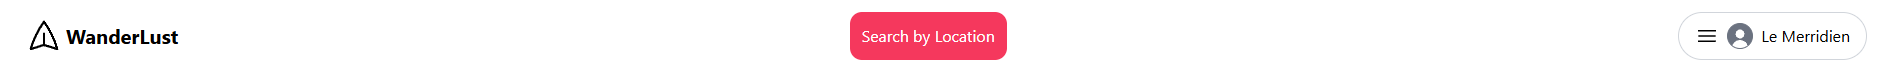
\includegraphics[width=\linewidth]{images/navbar.png} % Replace with your image file name
    \caption{Navbar}
    \label{fig:sample_image}
\end{figure}

\subsection{Home Page}
\begin{itemize}
    \item Listing of the properties with their main image, Title and Address.
    \item All the listings are clickable and it will navigate to that individual page details. From where the user can book that particular place.
\end{itemize}
\begin{figure}[h!]
    \centering
    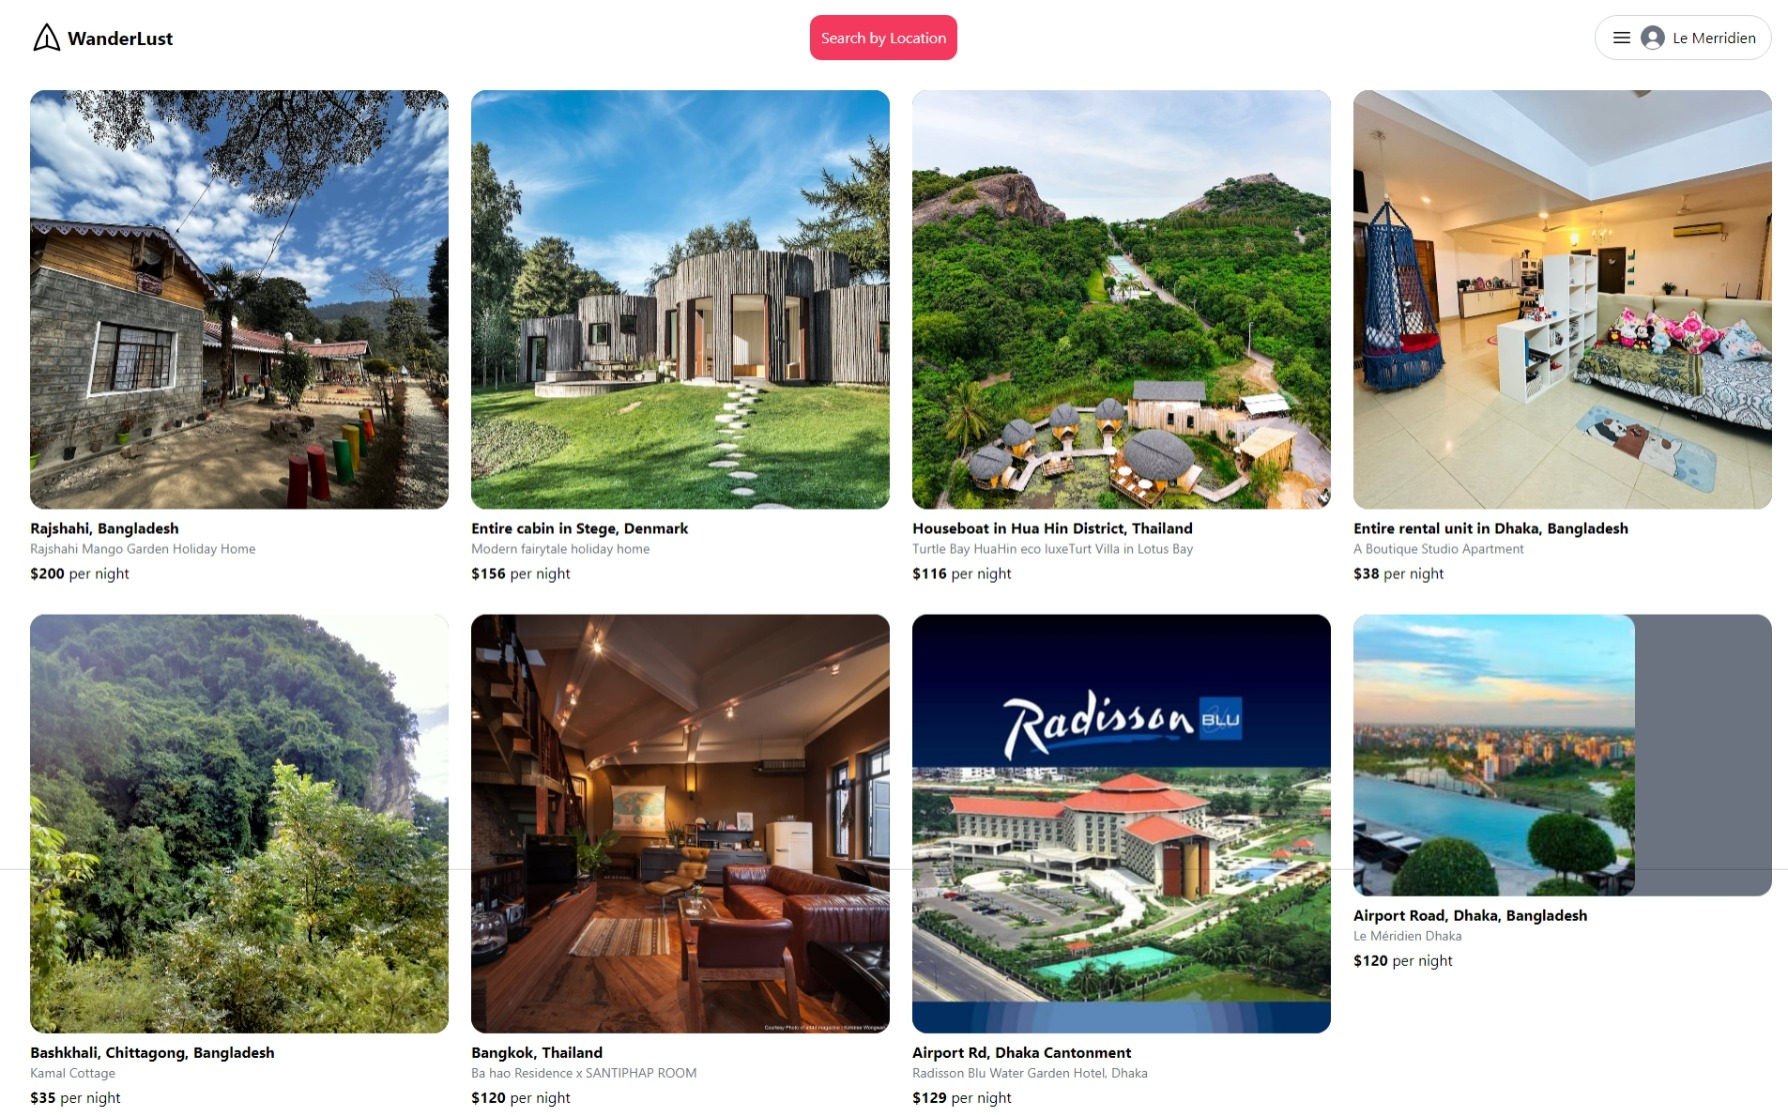
\includegraphics[width=\linewidth]{images/homepage.jpeg} % Replace with your image file name
    \caption{Home Page}
    \label{fig:sample_image}
\end{figure}
\subsection{Search Page}
\begin{itemize}
    \item When the user click the search button it will take the user to the search page. Where users can search the page by its location.
    \item If no matching places are found for the entered address, the message No results found is displayed in the results section.
    \item If results are found, this area would likely display a list or details of places matching the search query.
    \item The places will be clickable and will take the user to that particular place page.
\end{itemize}
\begin{figure}[h!]
    \centering
    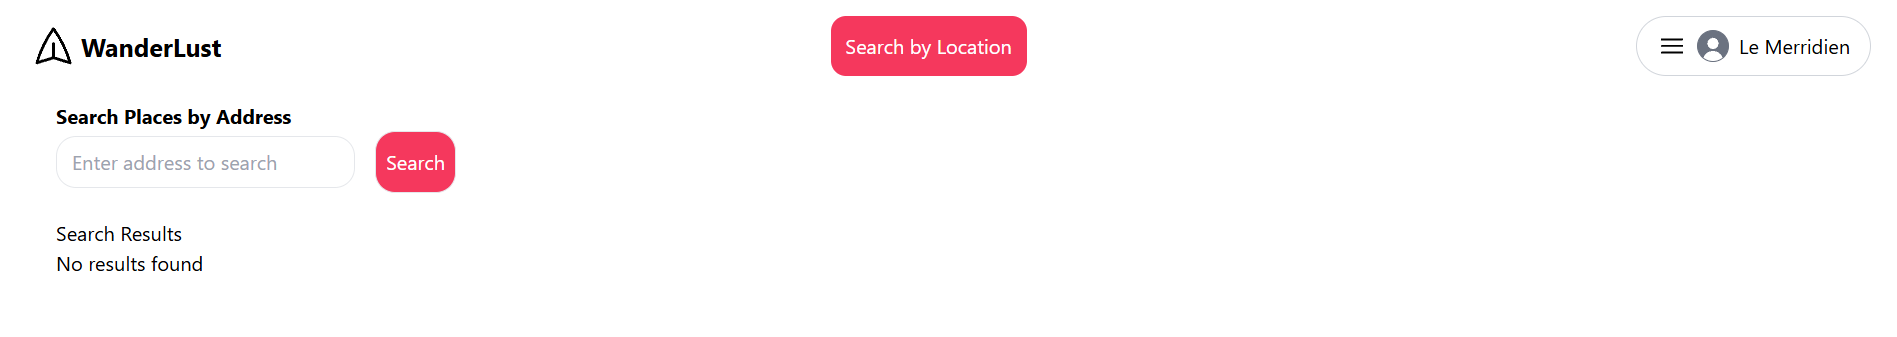
\includegraphics[width=\linewidth]{images/image.png} % Replace with your image file name
    \caption{Search Page}
    \label{fig:sample_image}
\end{figure}
\subsection{Login-Logout and Register}
\begin{itemize}
    \item A new user can register to the website, and their information (Name, Email, Encrypted Password) will be stored in the database.
    \item After registering, the user can log in to the website using their e-mail address and password.
    \item After finishing their session, they can log out from their account page.
\end{itemize}

\begin{figure}[H]
    \centering
    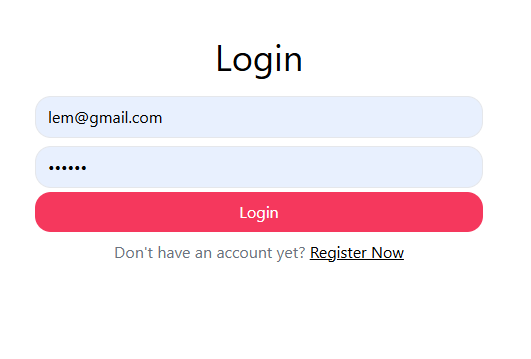
\includegraphics[width=\linewidth]{images/login.png} % Replace with your image file name
    \caption{Login Page}
    \label{fig:sample_image}
\end{figure}

\begin{figure}[H]
    \centering
    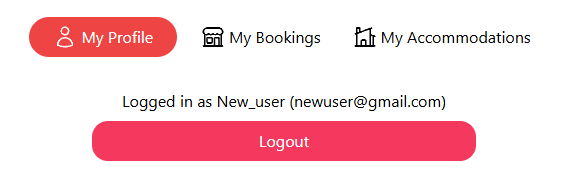
\includegraphics[width=\linewidth]{images/logout.png} % Replace with your image file name
    \caption{Logout Page}
    \label{fig:sample_image}
\end{figure}

\begin{figure}[H]
    \centering
    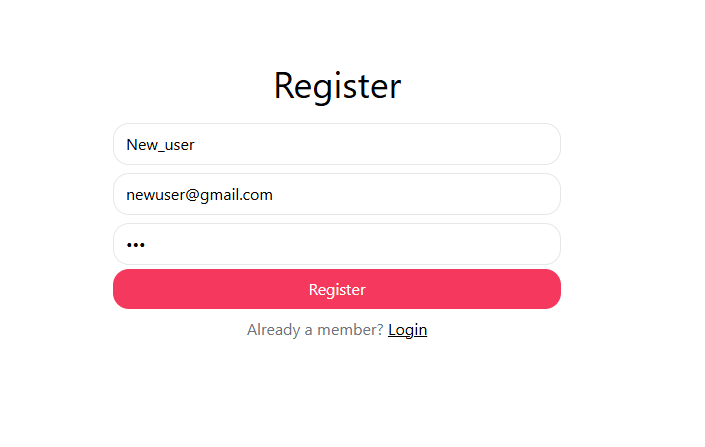
\includegraphics[width=\linewidth]{images/register.png} % Replace with your image file name
    \caption{Register Page}
    \label{fig:sample_image}
\end{figure}

\subsection{My Bookings}
\begin{itemize}
    \item Users will find their bookings in this page.
\end{itemize}
\begin{figure}[h!]
    \centering
    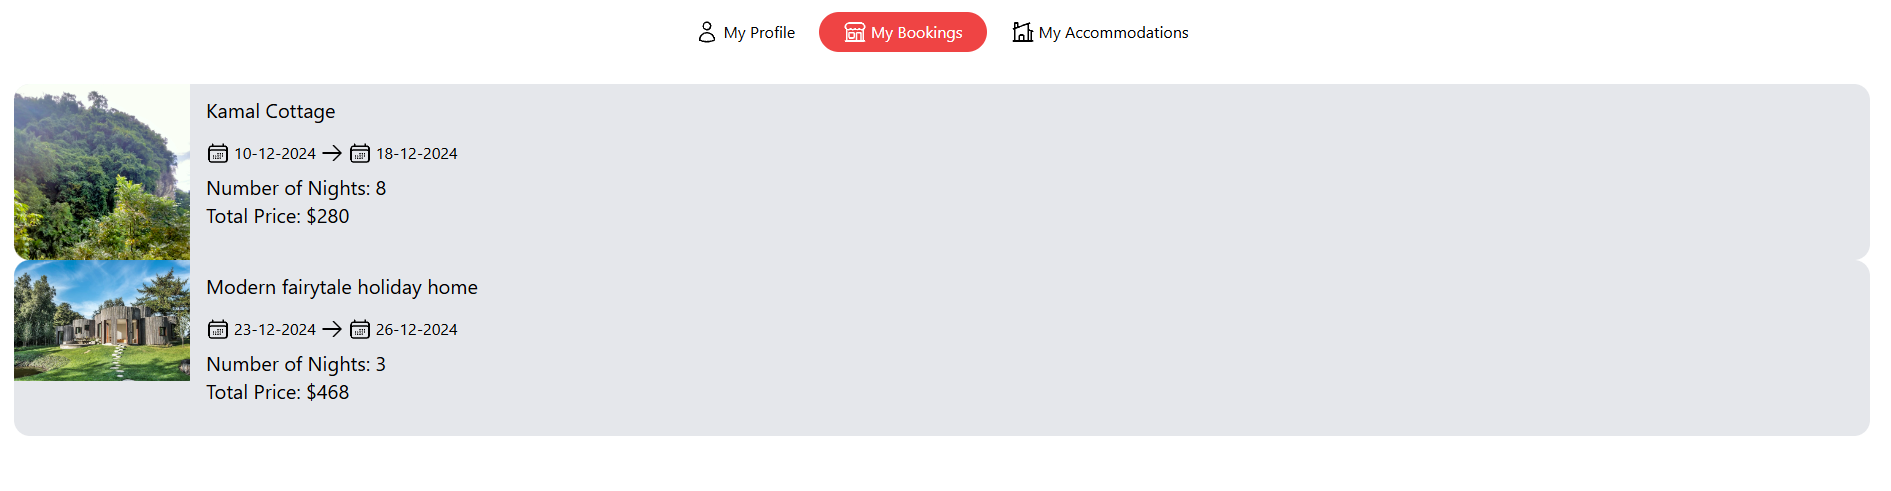
\includegraphics[width=\linewidth]{images/book.png} % Replace with your image file name
    \caption{My Bookings Page}
    \label{fig:sample_image}
\end{figure}
\subsection{My Accommodation}
\begin{itemize}
    \item Users will find their listed properties for rent in this page.
    \item •	They will also have a option of add a new place.
\end{itemize}
\begin{figure}[h!]
    \centering
    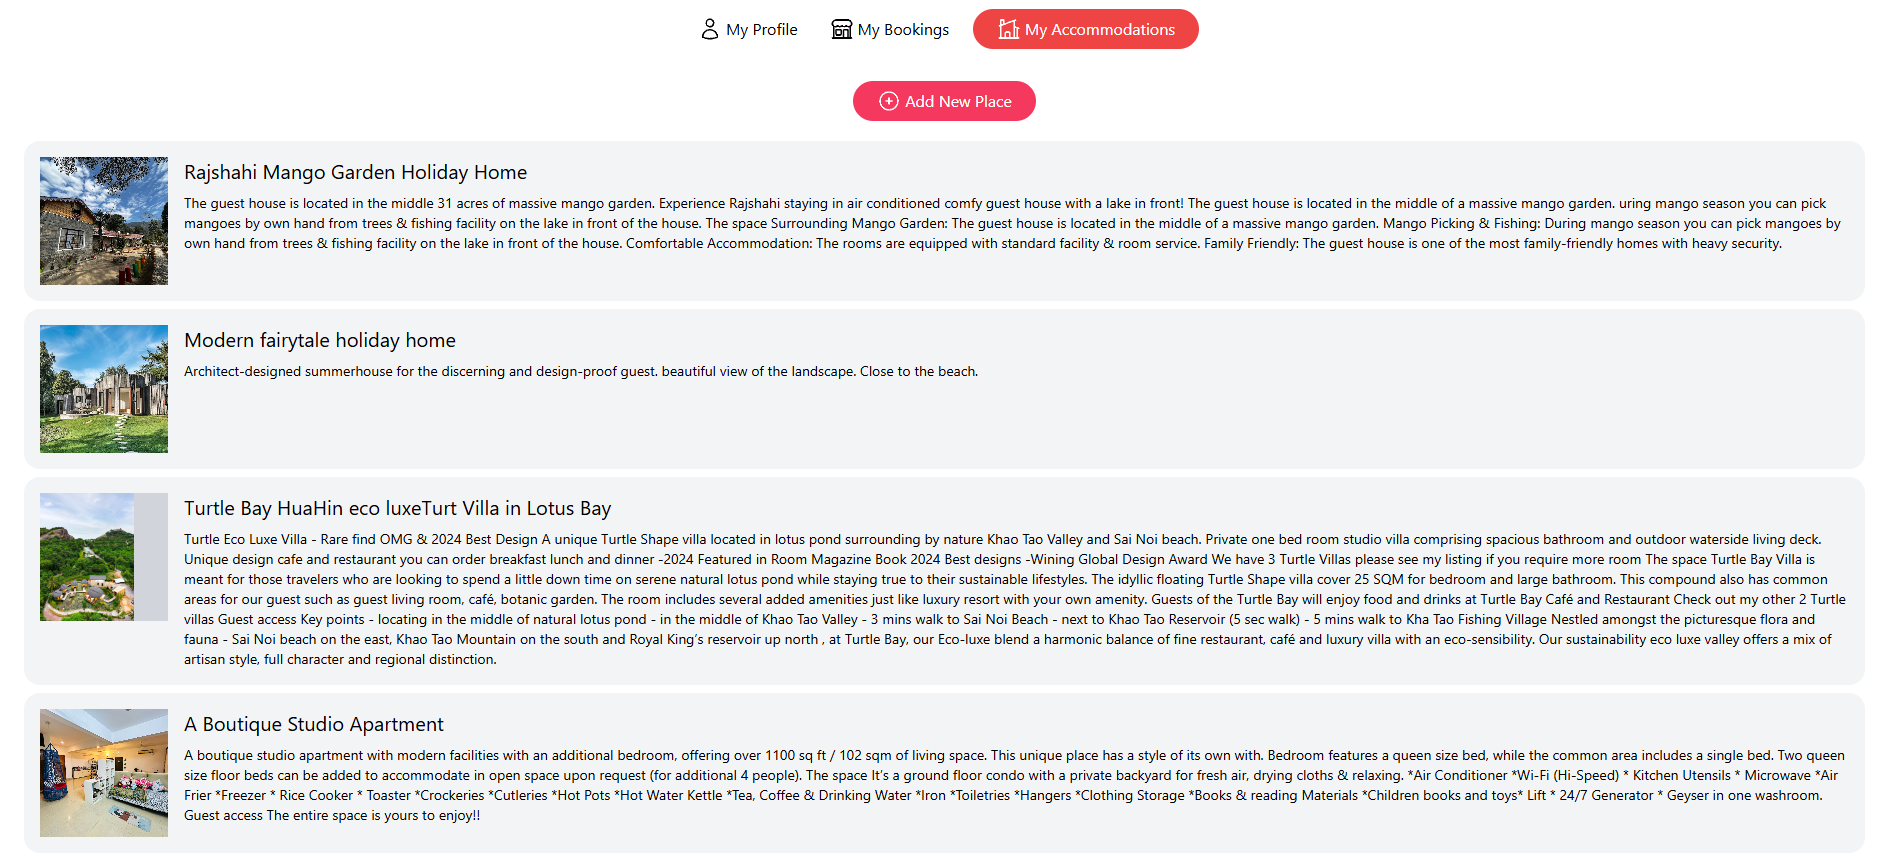
\includegraphics[width=\linewidth]{images/accom.png} % Replace with your image file name
    \caption{My Listed Accommodation Page}
    \label{fig:sample_image}
\end{figure}
\subsection{Individual Place’s Page}
\begin{itemize}
    \item This page will show the details of that place.
    \item Their address is clickable and it will navigate to the google map of that location.
    \item Three photos will be visible in this page. If user wants to see more photos they can click any of the photos or tap the Show More Photos Button
    \item  Main Booking functionality will happen in this page. Logged in user can book this place.
    \item While booking, user must enter their dates, Number of Guests. After inserting the dates, the price and name of the Guest will automatically appeared on the booking widget.
    \item User can also find the description, perks and extra info of this place.
\end{itemize}
\begin{figure}[H]
    \centering
    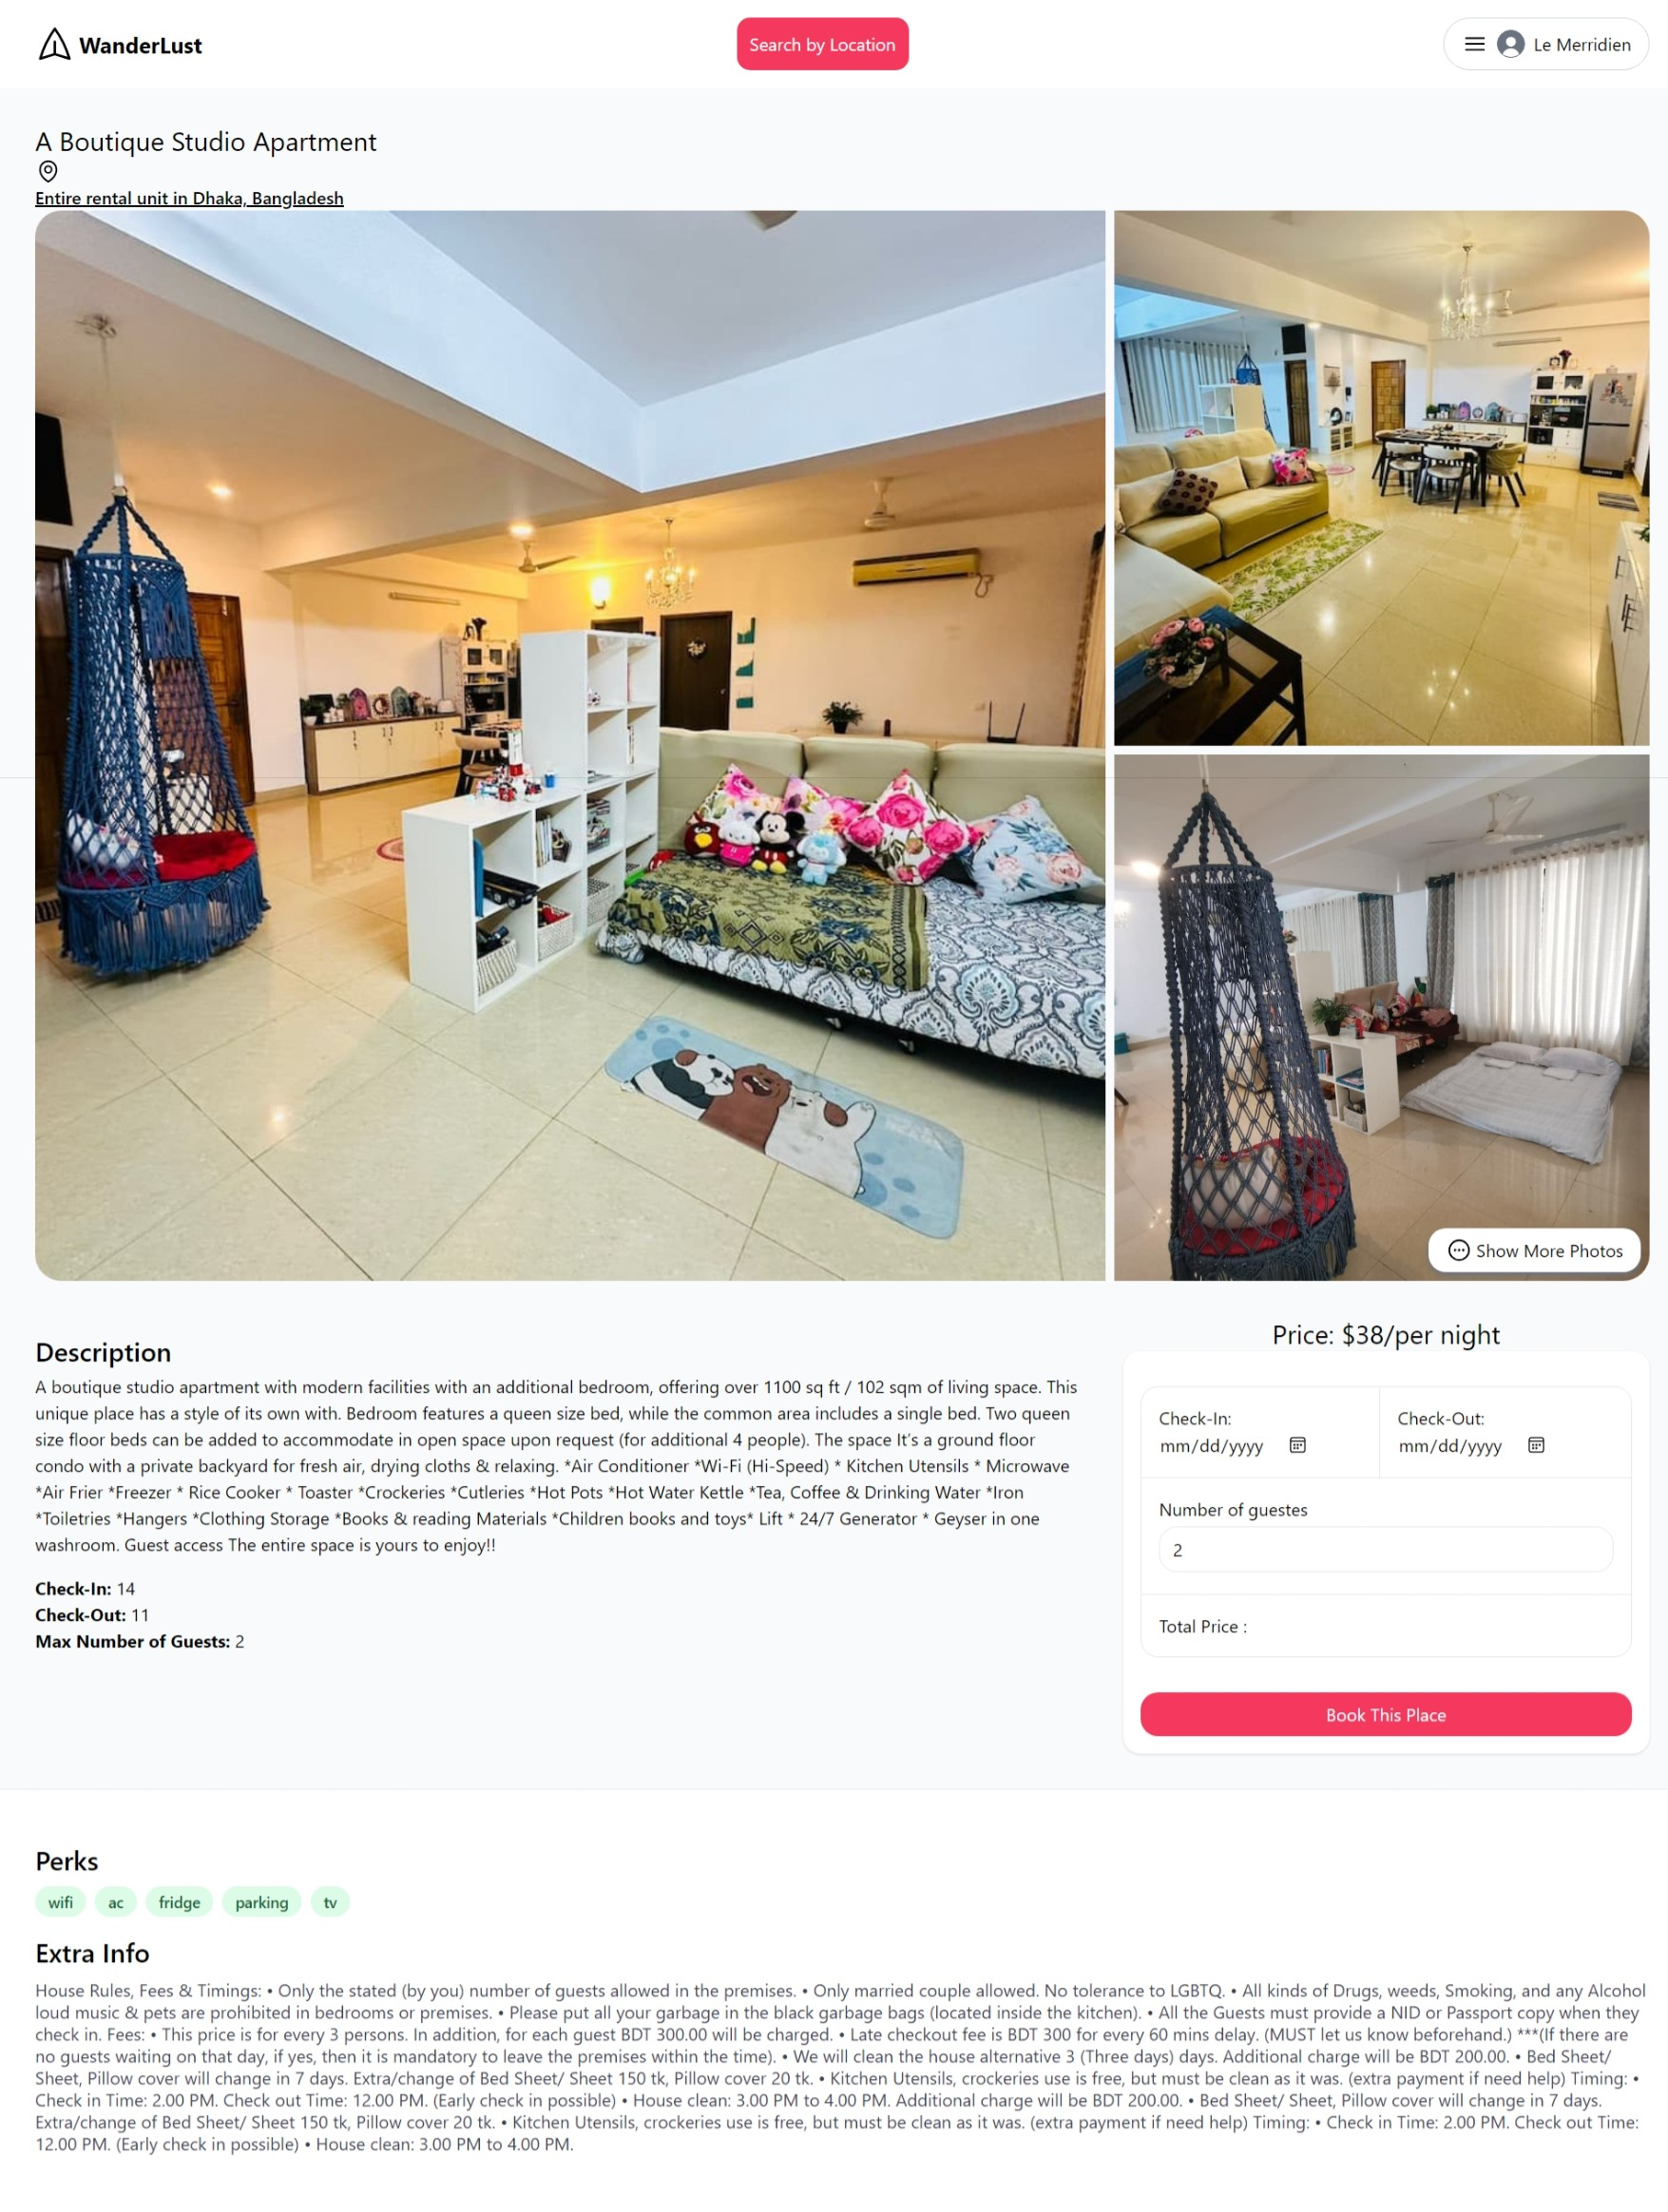
\includegraphics[width=\linewidth]{images/placepage.jpeg} % Replace with your image file name
    \caption{Individual Place’s Page}
    \label{fig:sample_image}
\end{figure}
\subsection{Booking Confirmed Page}
\begin{itemize}
    \item When user will book a place through Individual Place’s Page, it will redirect to booking confirmation page.
    \item This page can also be accessed from user’s booked place from their account page.
    \item If user wishes they can cancel this booking from this page.
\end{itemize}
\begin{figure}[H]
    \centering
    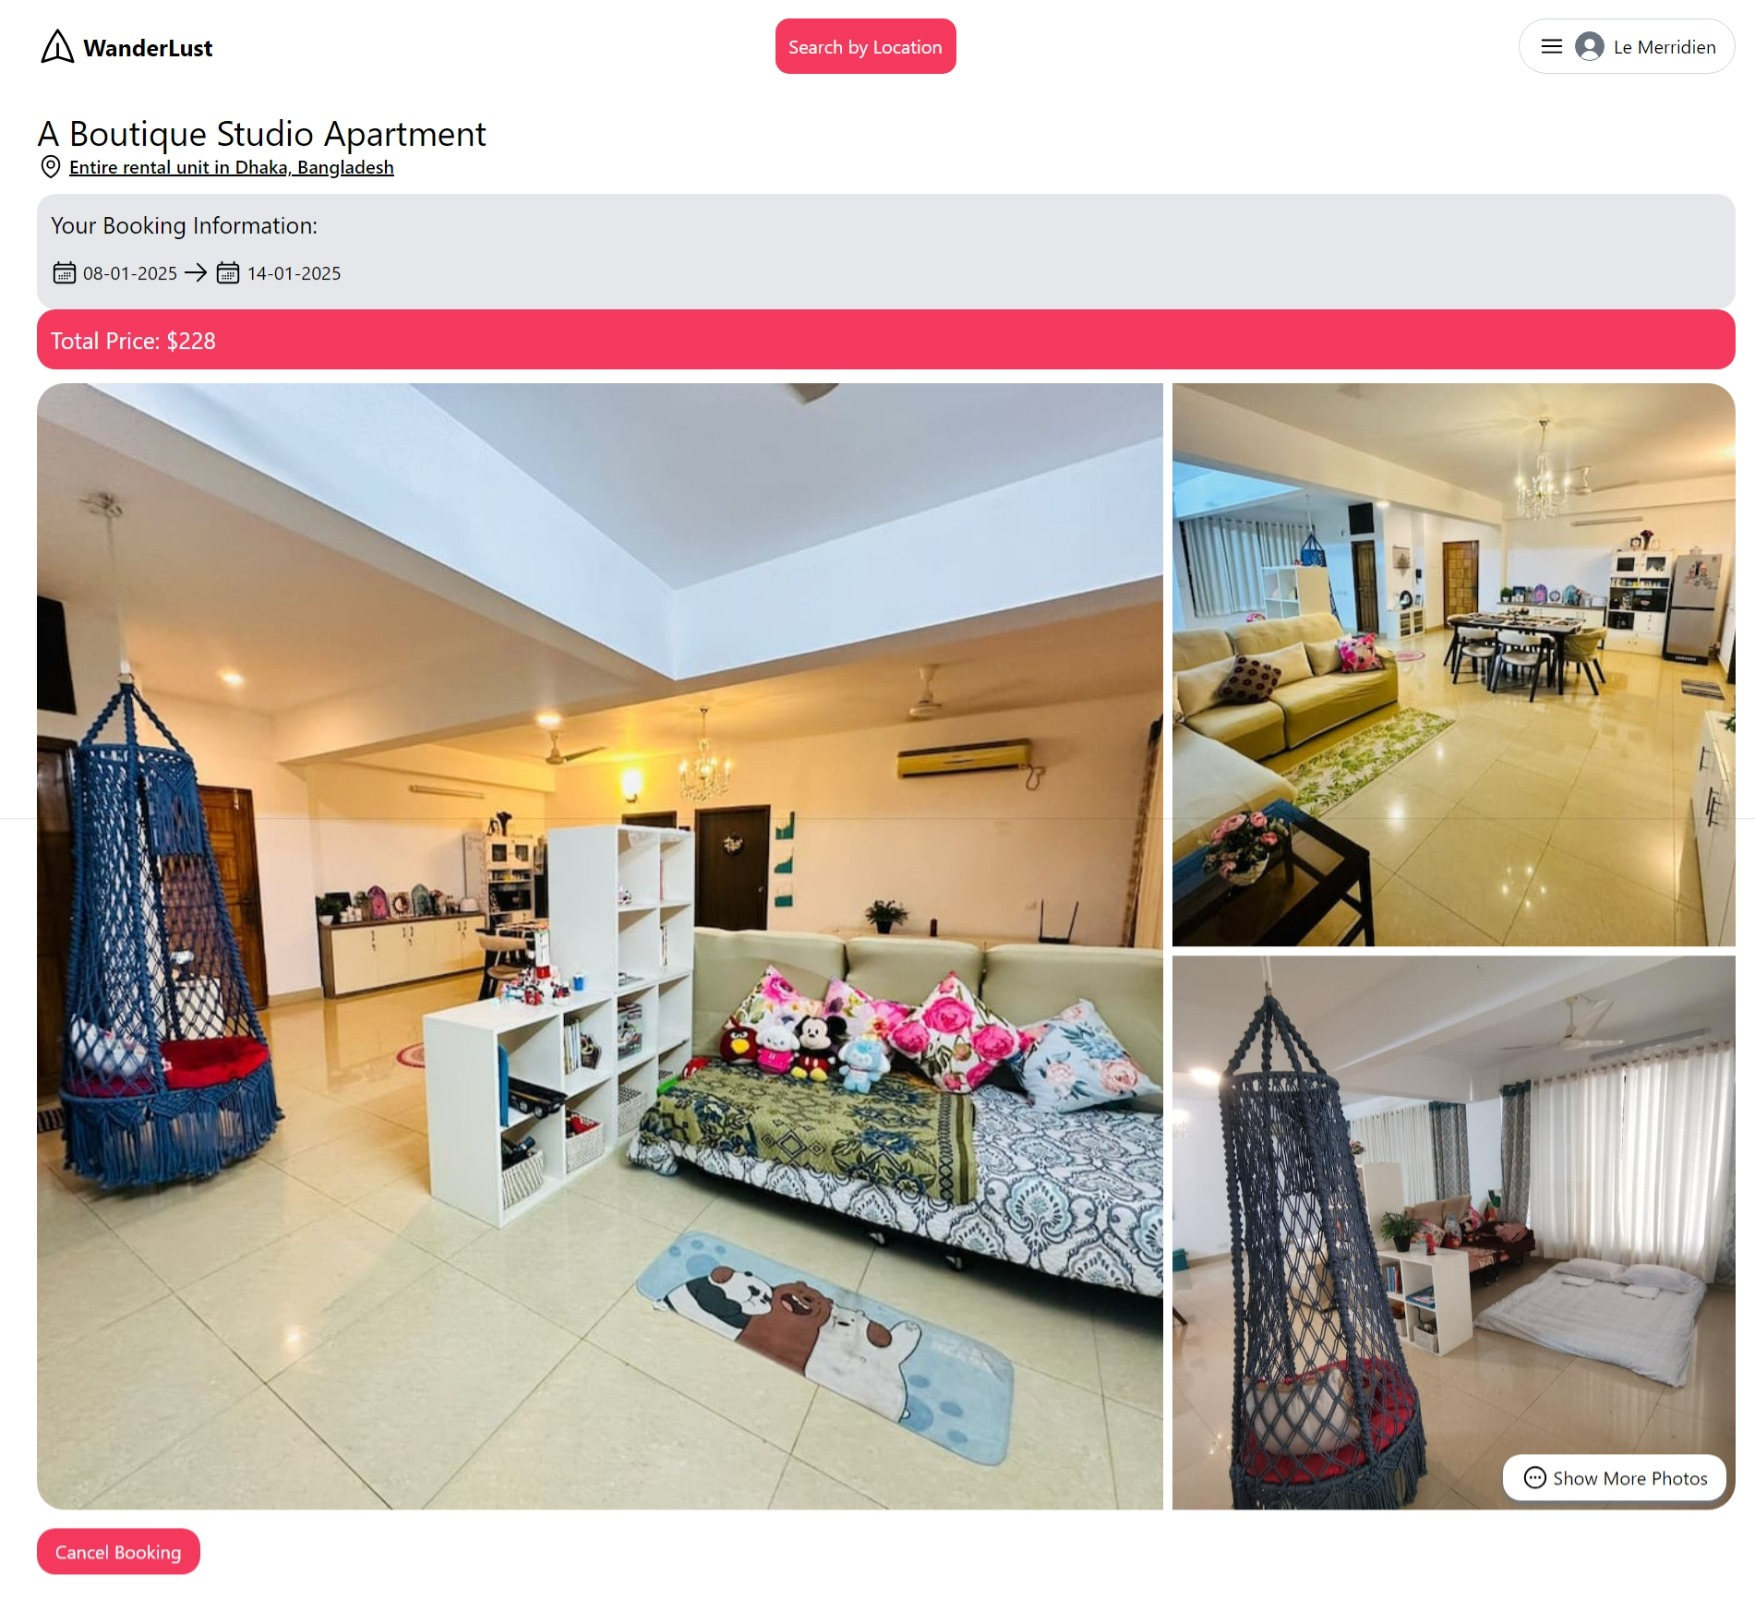
\includegraphics[width=\linewidth]{images/bookingpage.jpeg} % Replace with your image file name
    \caption{Booking Confirmed Page}
    \label{fig:sample_image}
\end{figure}
\section{Main Differentiator}
The main difference between my website, WanderLust, and other hotel booking platforms like Booking.com, Agoda.com, and Trivago.com is that those websites do not allow individual users to list properties. However, on WanderLust, any registered user can list a single apartment, as well as large hotels, providing more flexibility in property listings.
\begin{figure}[H]
    \centering
    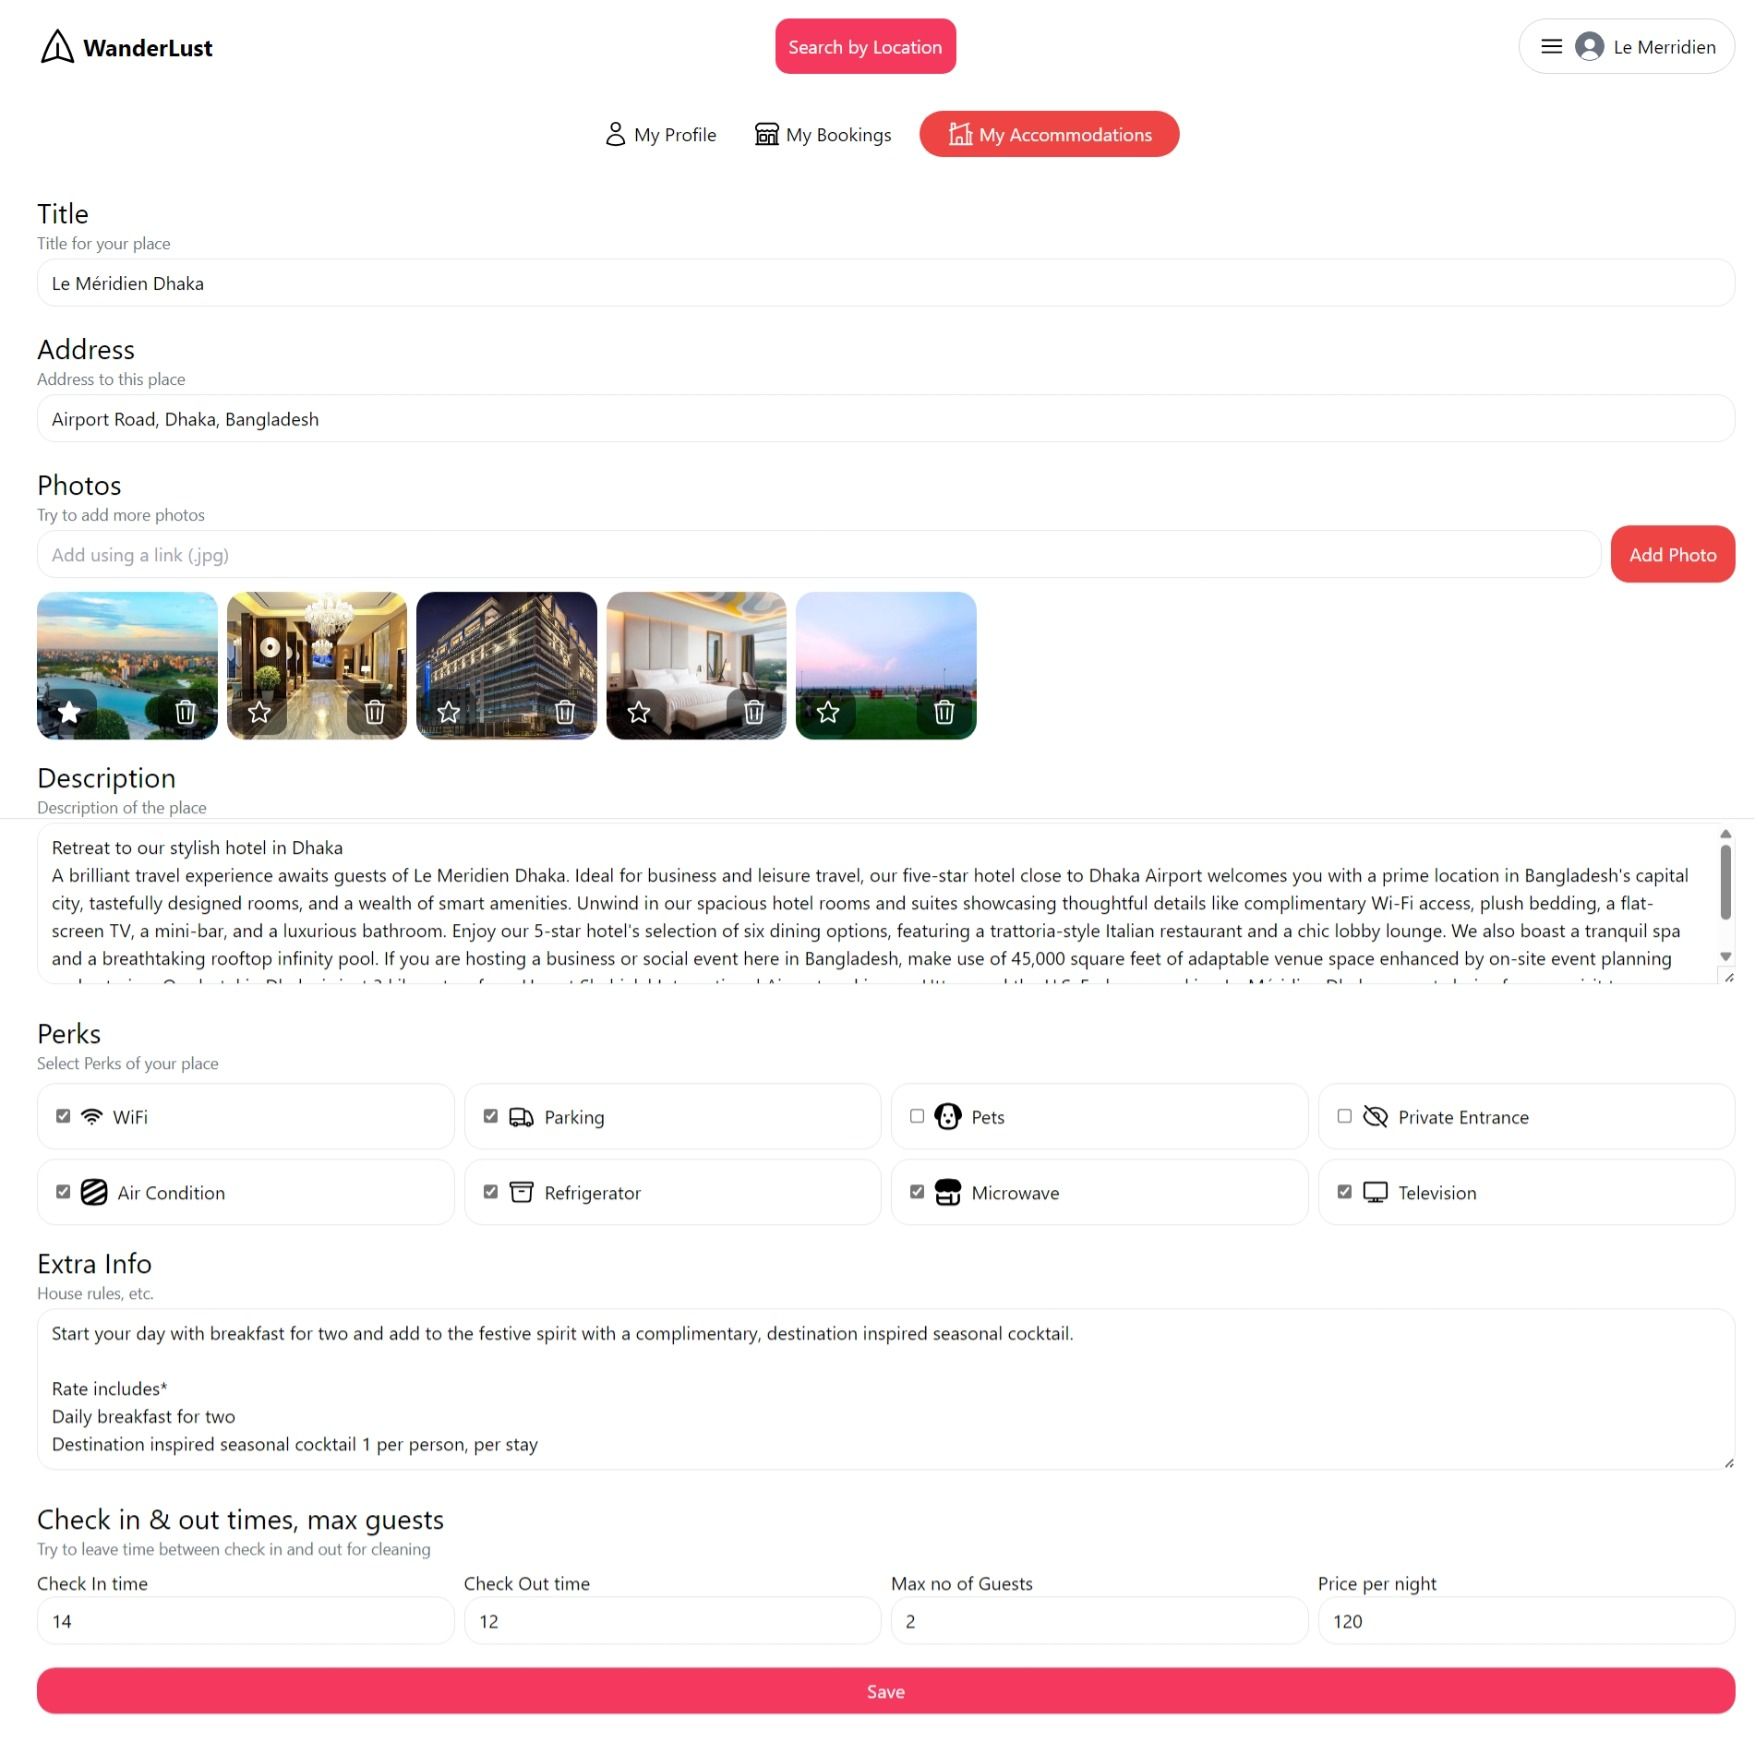
\includegraphics[width=\linewidth]{images/listing.jpeg} % Replace with your image file name
    \caption{Listing Page}
    \label{fig:sample_image}
\end{figure}

\section{New Feature: Filtered Search Functionality}
A new feature has been integrated into the WanderLust platform: \textbf{Filtered Search}. This enhancement significantly improves the user experience by allowing travelers to refine their accommodation search results based on specific preferences.

\subsection*{Key Functionalities}
\begin{itemize}
    \item Users can now filter search results by:
    \begin{itemize}
        \item Price range
        \item Number of guests
        \item Availability dates
        \item Amenities (e.g., Wi-Fi, air conditioning, pet-friendly, parking)
    \end{itemize}
    \item Filters can be applied on the Search Page after entering a destination or location.
    \item The page dynamically updates the displayed results based on the selected filters, providing a tailored browsing experience.
    \item If no results match the applied filters, a message stating \texttt{No results found} will appear.
\end{itemize}

\subsection*{Benefits}
\begin{itemize}
    \item Enhances usability and user satisfaction by offering a more personalized search experience.
    \item Helps users quickly find properties that meet their exact needs, reducing the time spent scrolling through irrelevant listings.
    \item Empowers hosts to better highlight unique amenities and features of their properties.
\end{itemize}

\begin{figure}[H]
    \centering
    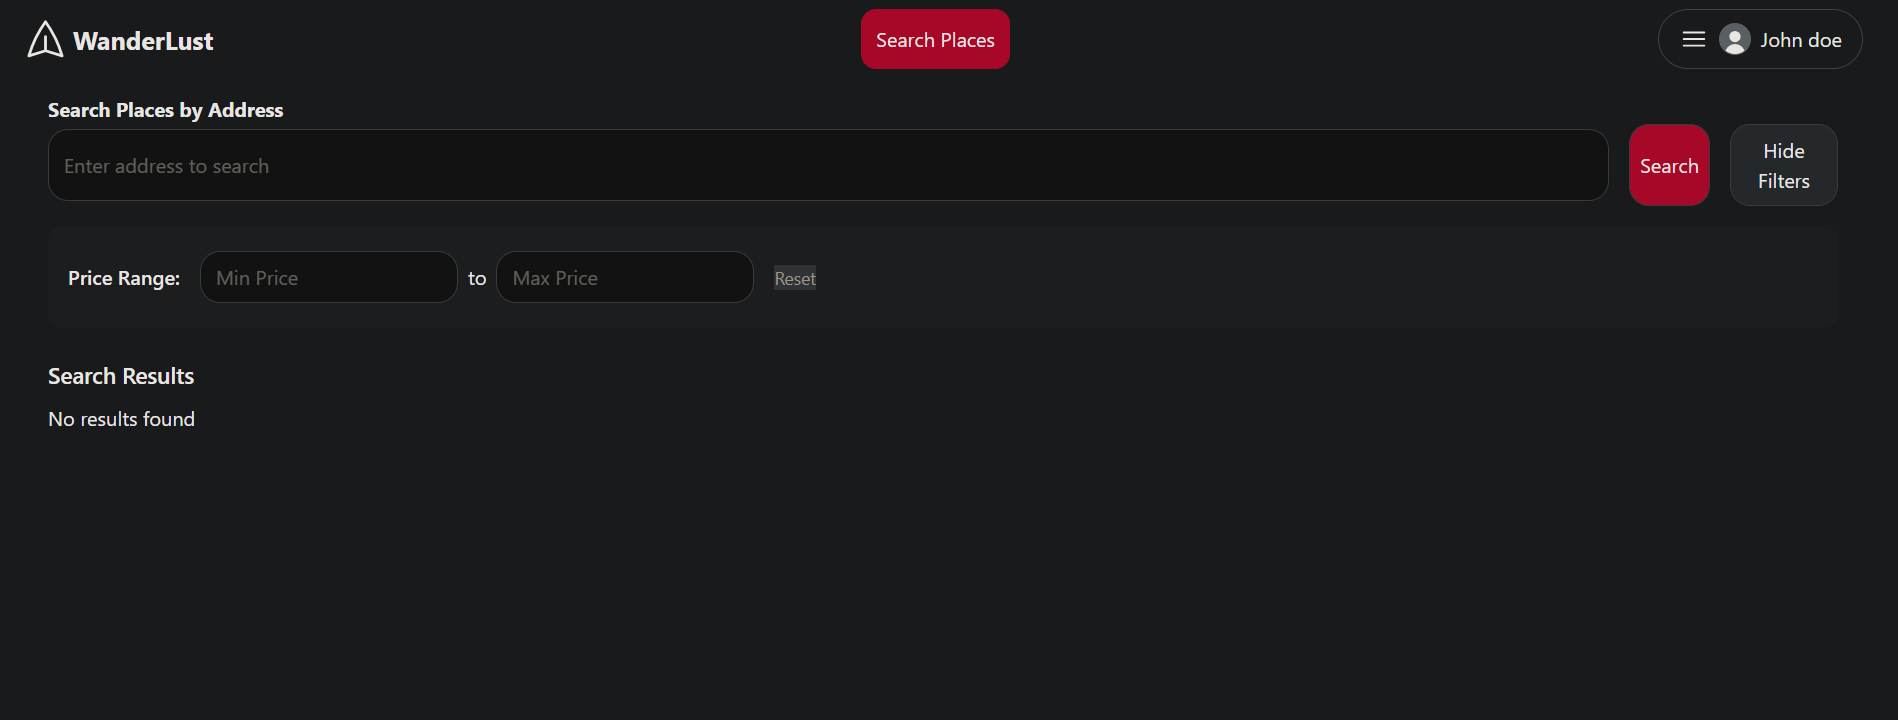
\includegraphics[width=\linewidth]{images/fil1.png} % Replace with your image file name
    \caption{Filtered Search Page}
    \label{fig:filtered_search}
\end{figure}

\begin{figure}[H]
    \centering
    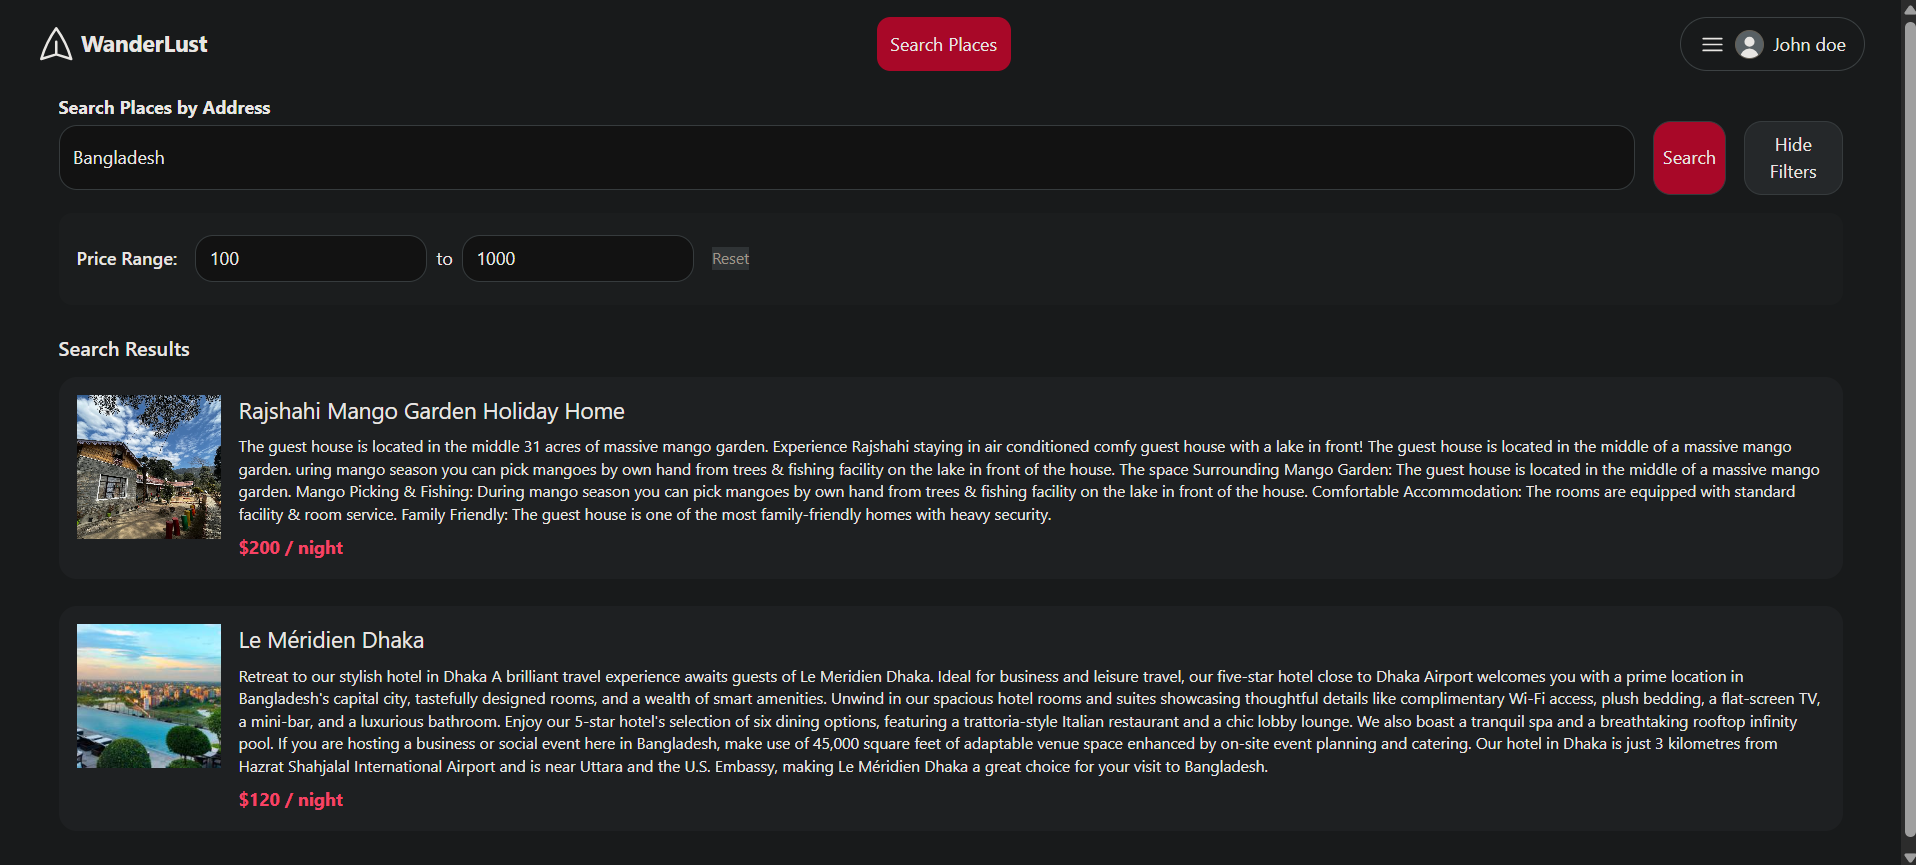
\includegraphics[width=\linewidth]{images/fil2.png} % Replace with your image file name
    \caption{Filtered Search Results}
    \label{fig:filtered_search}
\end{figure}


\section{GitHub Upload}
This project is uploaded to GitHub using these following commands:
\begin{verbatim}
    # Initialize Git in my project directory
    git init
    
    # Add all files to the staging area
    git add .
    
    # Commit the files with a meaningful message
    git commit -m "Initial commit for WanderLust project"
    
    # Create a new repository on GitHub named 'WanderLust'
    # Linking local repository to the remote GitHub repository
    git remote add origin https://github.com/RafinEazdan/WanderLust.git
    
    # Push the local repository to GitHub
    git branch -M main
    git push -u origin main
    \end{verbatim}
    \begin{figure}[H]
        \centering
        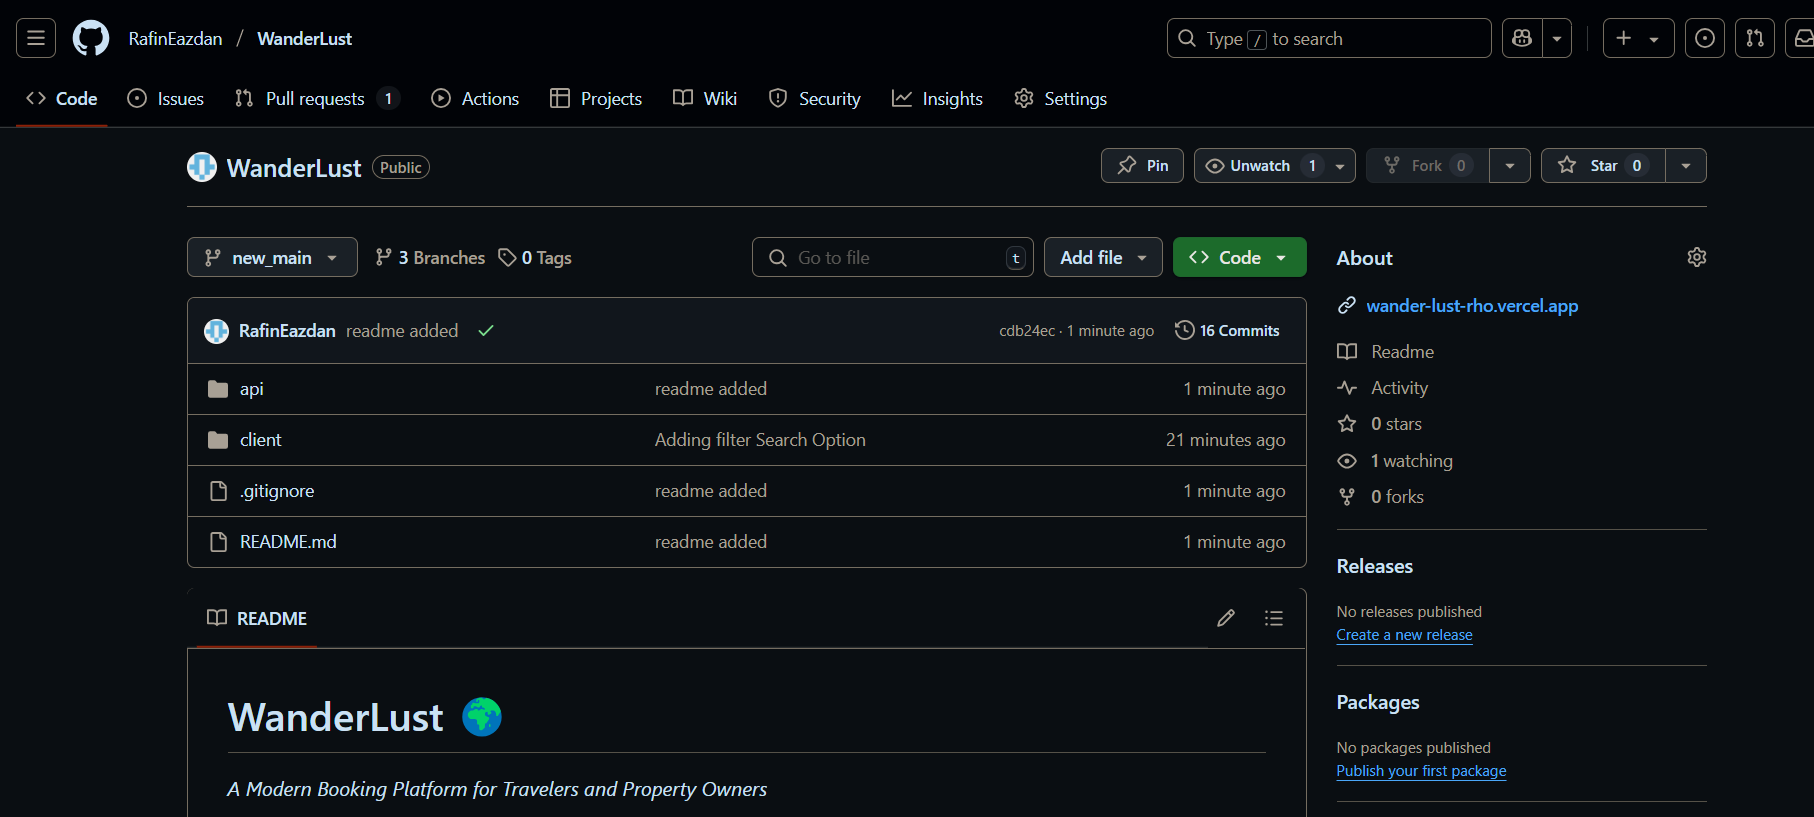
\includegraphics[width=\linewidth]{images/Git.png} % Replace with your image file name
        \caption{Github Repository}
        \label{fig:sample_image}
    \end{figure}
\section{Technology Stack}
\subsection{Backend}
The backend is powered by modern technologies, ensuring robust and secure handling of user data, property information, and bookings. Technologies used include:
\begin{itemize}
    \item JavaScript
    \item Node.js
    \item MongoDB for NoSQL database management
    \item Express.js
    \item Bcryptjs for encrypting password
    \item Dotenv for managing env files
    \item Cookie-Parser is used to parse cookies attached to the incoming request object.
\end{itemize}

\subsection{Frontend}
The frontend is designed to provide an intuitive and responsive user interface. Technologies used include:
\begin{itemize}
    \item HTML
    \item Tailwind CSS for styling
    \item JavaScript
    \item Vite
    \item Yarn instead of NPM for better performance while installing packages
    \item ReactJS
    \item React-router-dom
    \item Axios
\end{itemize}

\section{Conclusion}
WanderLust connects travelers with property owners, offering a wide range of accommodations from low-cost stays to luxurious retreats. It improves the vacation experience by providing a user-friendly platform that allows hosts to maximize the potential of their properties.
\end{document}
